\FloatBarrier
\section{Durchführung}
\label{sec:Durchführung}

Um die Suszeptibilität paramagnetischer Stoffe experimentell bestimmen zu können, wird eine Brückenschaltung verwendet.
Der Aufbau dieser ist in Abbildung \ref{fig:Brückenschaltung} dargestellt.
Wie in Abschnitt \ref{sec:praktischeTheorie} sind die bei diesem Aufbau auftretenden Brückenspannungen in der Größenordnung der Störspannungen.
Es sind daher einige Maßnahmen nötig um die Brückenspannungen auswerten zu können und somit die Suszeptibilität ausrechnen zu können.
Der grobe Aufbau ist in Abbildung \ref{fig:Aufbau} gezeigt.

\begin{figure}
  \centering
  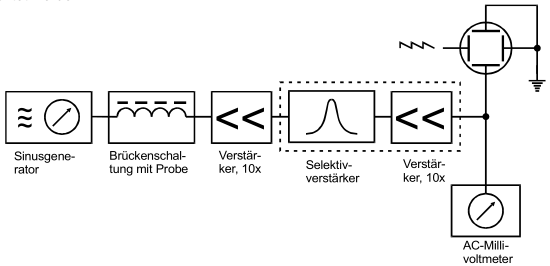
\includegraphics[width=0.75\textwidth]{images/Aufbau.png}
  \caption{Maßnahmen, um die Brückenspannung vernünftig isolieren zu können, entnommen der Versuchsanleitung\cite[183]{sample}}
  \label{fig:Aufbau}
\end{figure}

 Am wichtigsten zum Isolieren der Brückenspannung ist der bereits erwähnte Selektivverstärker.
 Er ermöglicht es die monofrequente Brückenspannung aus der breitbandigen Störspannung hinreichend genau zu isolieren.
 Eine beispielhafte Filterkurve ist in Abbildung \ref{fig:theofilterkurve} dargestellt.
 Die dort erwähnte Güte gibt die entsprechende Weite der Kurve an.
 Diese wird für diesen Versuch auf $Q = 100$ eingestellt.

 Die Filterkurve wird zur Verifizierung dieses Wertes untersucht.
 Dafür wird ein Synthesizer direkt mit dem Selektivverstärker verbunden.
 Die Durchlassfrequenz des Selektivverstärker wird auf einen Wert zwischen $30 - \SI{40}{\kilo\hertz}$ eingestellt.
 Bei konstanter Eingangsspannung von maximal $\SI{1}{\volt}$ wird dann die Ausgangsspannung in Abhängigkeit von der Frequenz zwischen $30 - \SI{40}{\kilo\hertz}$ gemessen.

Zur Bestimmung der eigentlichen Suszeptibilität werden die Elemente gemäß Abbildung \ref{fig:Aufbau} aufgebaut.

Brb!
